
\slidesectionwithgraphic{About Us}{images/aboutus}


\begin{frame}{Computer Graphics Systems at HPI}

    \vfill
	\LARGE
	\blueify{Chair for \textit{\enquote{Design, Analysis, and Construction of Computer Graphics Systems}}}

	\bigskip
	\bigskip
	\normalsize
	\textbf{Fields of Research}
	\begin{itemize}
		\item 3D Computer Graphics (Rendering, Middleware, Content Management)  
		\item Image \& Video (Nonphotorealism, Video Analytics, Video Abstracion)
		\item Software Analytics (Software Maps, Software Metrics, System Evolution)	
		\item Service-Oriented Architectures for Computer Graphics Systems		
	\end{itemize}
	
	\vfill
\end{frame}


\begin{frame}[fragile]{Computer Graphics Systems at HPI | \textbf{Curriculum}}

    \vfill\centering\small

	{ \def\arraystretch{1.2}
	
	\begin{tabular}{l|l|l}
		\multicolumn{3}{c}{\Large \grayout{Bachelor IT-Systems Engineering}} \medskip\\

		\blueify{\normalsize Lectures} & \blueify{\normalsize Seminars} & \blueify{\normalsize Projects} \medskip\\
		3D Computer Graphics I & Graphics Programming (C++, OpenGL) & Bachelor Software Project \\
		3D Computer Graphics II & Introduction to Visual Analytics & Bachelor Thesis \\
		Programming Techniques II & Image and Video Processing & Software Development Projects \bigskip\bigskip\\
		
		\multicolumn{3}{c}{\Large \grayout{Master IT-Systems Engineering}} \medskip\\

		\blueify{\normalsize Lectures} & \blueify{\normalsize Seminars} & \blueify{\normalsize Projects} \medskip\\
		Advanced Programming in C++ & Software Analytics & Master Software Project \\
		Software Analytics & Geospatial Visual Analytics & Master Thesis \\
		Visualization & Image and Video Analytics & Software Development Projects \\
		Geovisualization & Information Visualization Techniques & \\
		Image and Video Processing & Advanced Development in C++ &

	\end{tabular}
	}
    \vfill
	
\end{frame}


\begin{frame}{Computer Graphics Systems at HPI | \textbf{Built Systems 1/4}}

	\begin{figure}
		\raggedright
		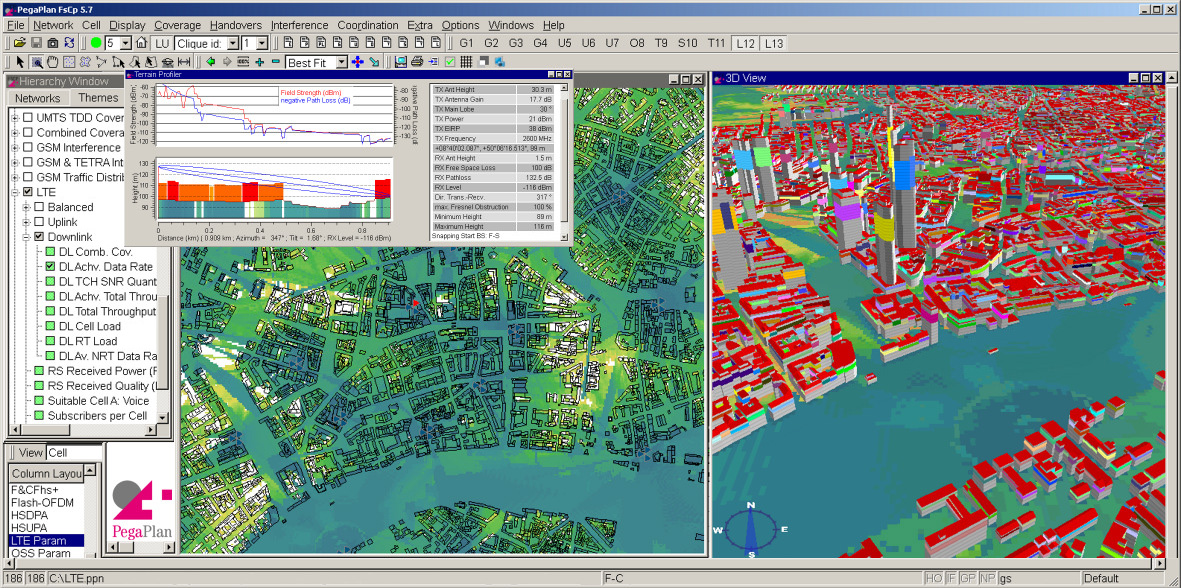
\includegraphics[height=0.32\textwidth]{images/pegaplan.jpg}
%		\caption{\scriptsize{User Interface of PegaPlan \url{http://www.pegaware.com/news/news-single/aktuell/see-pegaplan-lte-world-summit-2011.html}}}
	\end{figure}
	
	\blueify{PegaPlan Radio Network Planning System (T-Systems)}
	
	\begin{itemize}
		\item Interactive exploration and reconfiguration of radio networks
		\item Radio network optimization and simulation
		\item Step-by-step integration into the operational system of T-Mobile
	\end{itemize}
	
\end{frame}


\begin{frame}{Computer Graphics Systems at HPI | \textbf{Built Systems 2/4}}

	\begin{figure}
		\raggedright
		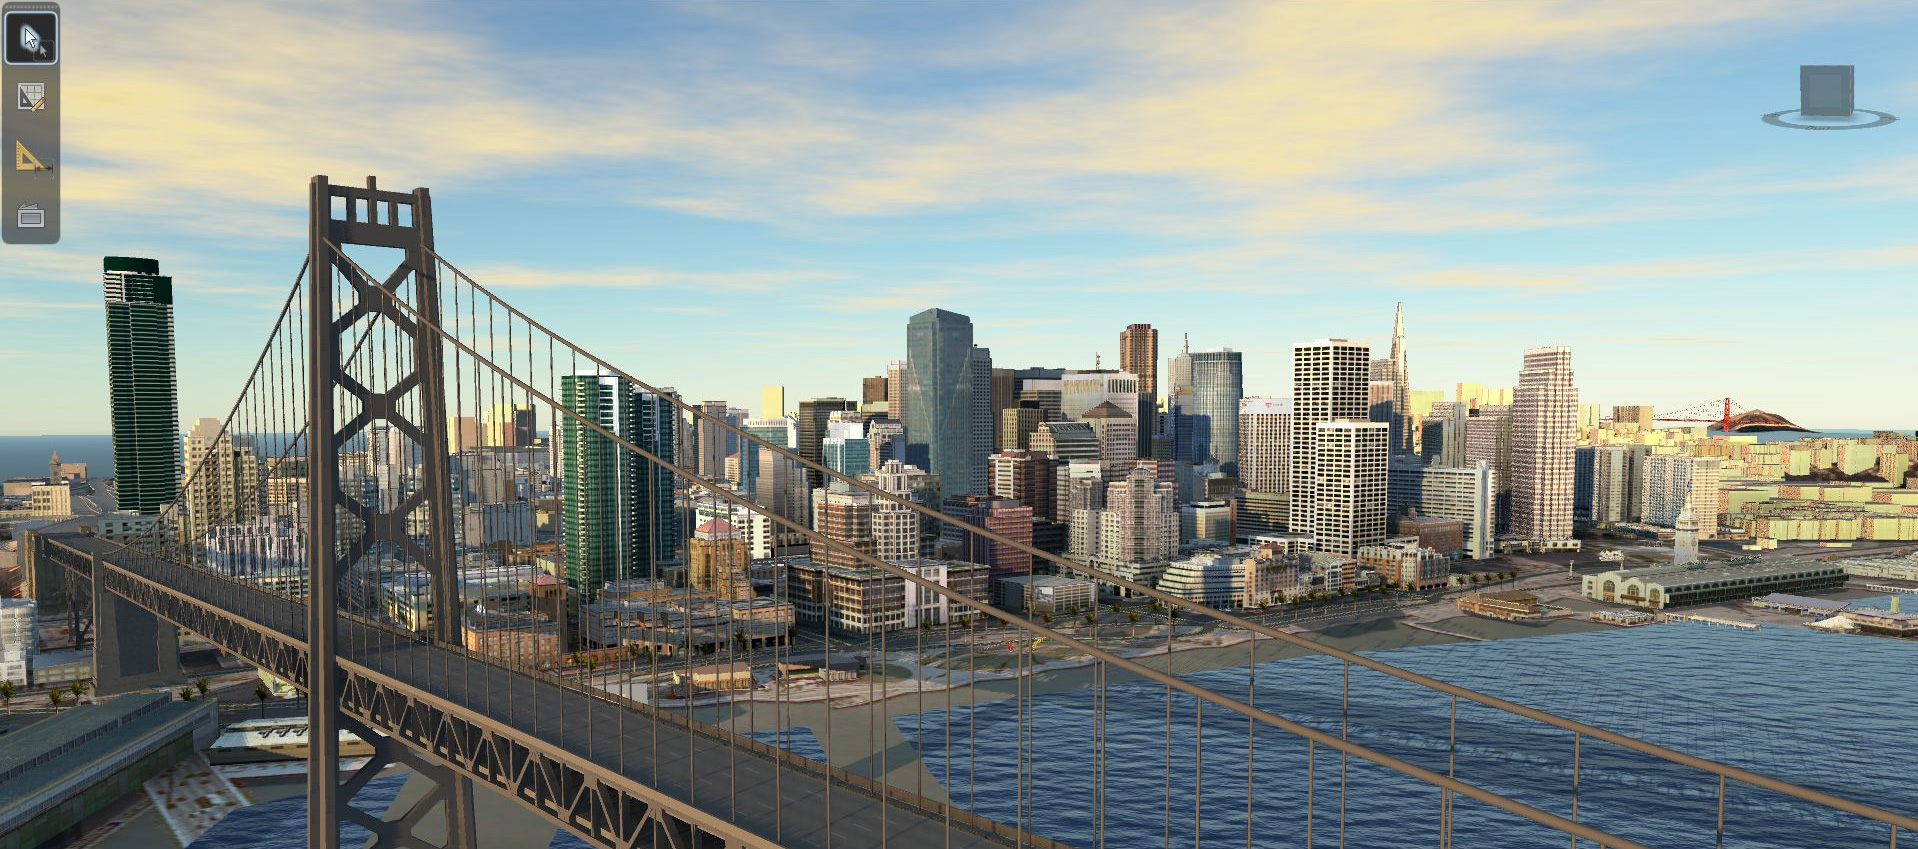
\includegraphics[height=0.32\textwidth]{images/infraworks}
	\end{figure}
	
	\blueify{LandXplorer (Autodesk Infraworks)}

	\begin{itemize}
		\item Interactive management and visualization of virtual 3D city models
		\item Real-time 3D rendering of massive 3D models
		\item Dedicated to \enquote{plan, design and engineer with real data, in the real world, in real time}
	\end{itemize}
	
\end{frame}


\begin{frame}{Computer Graphics Systems at HPI | \textbf{Built Systems 3/4}}

    \begin{figure}
 	   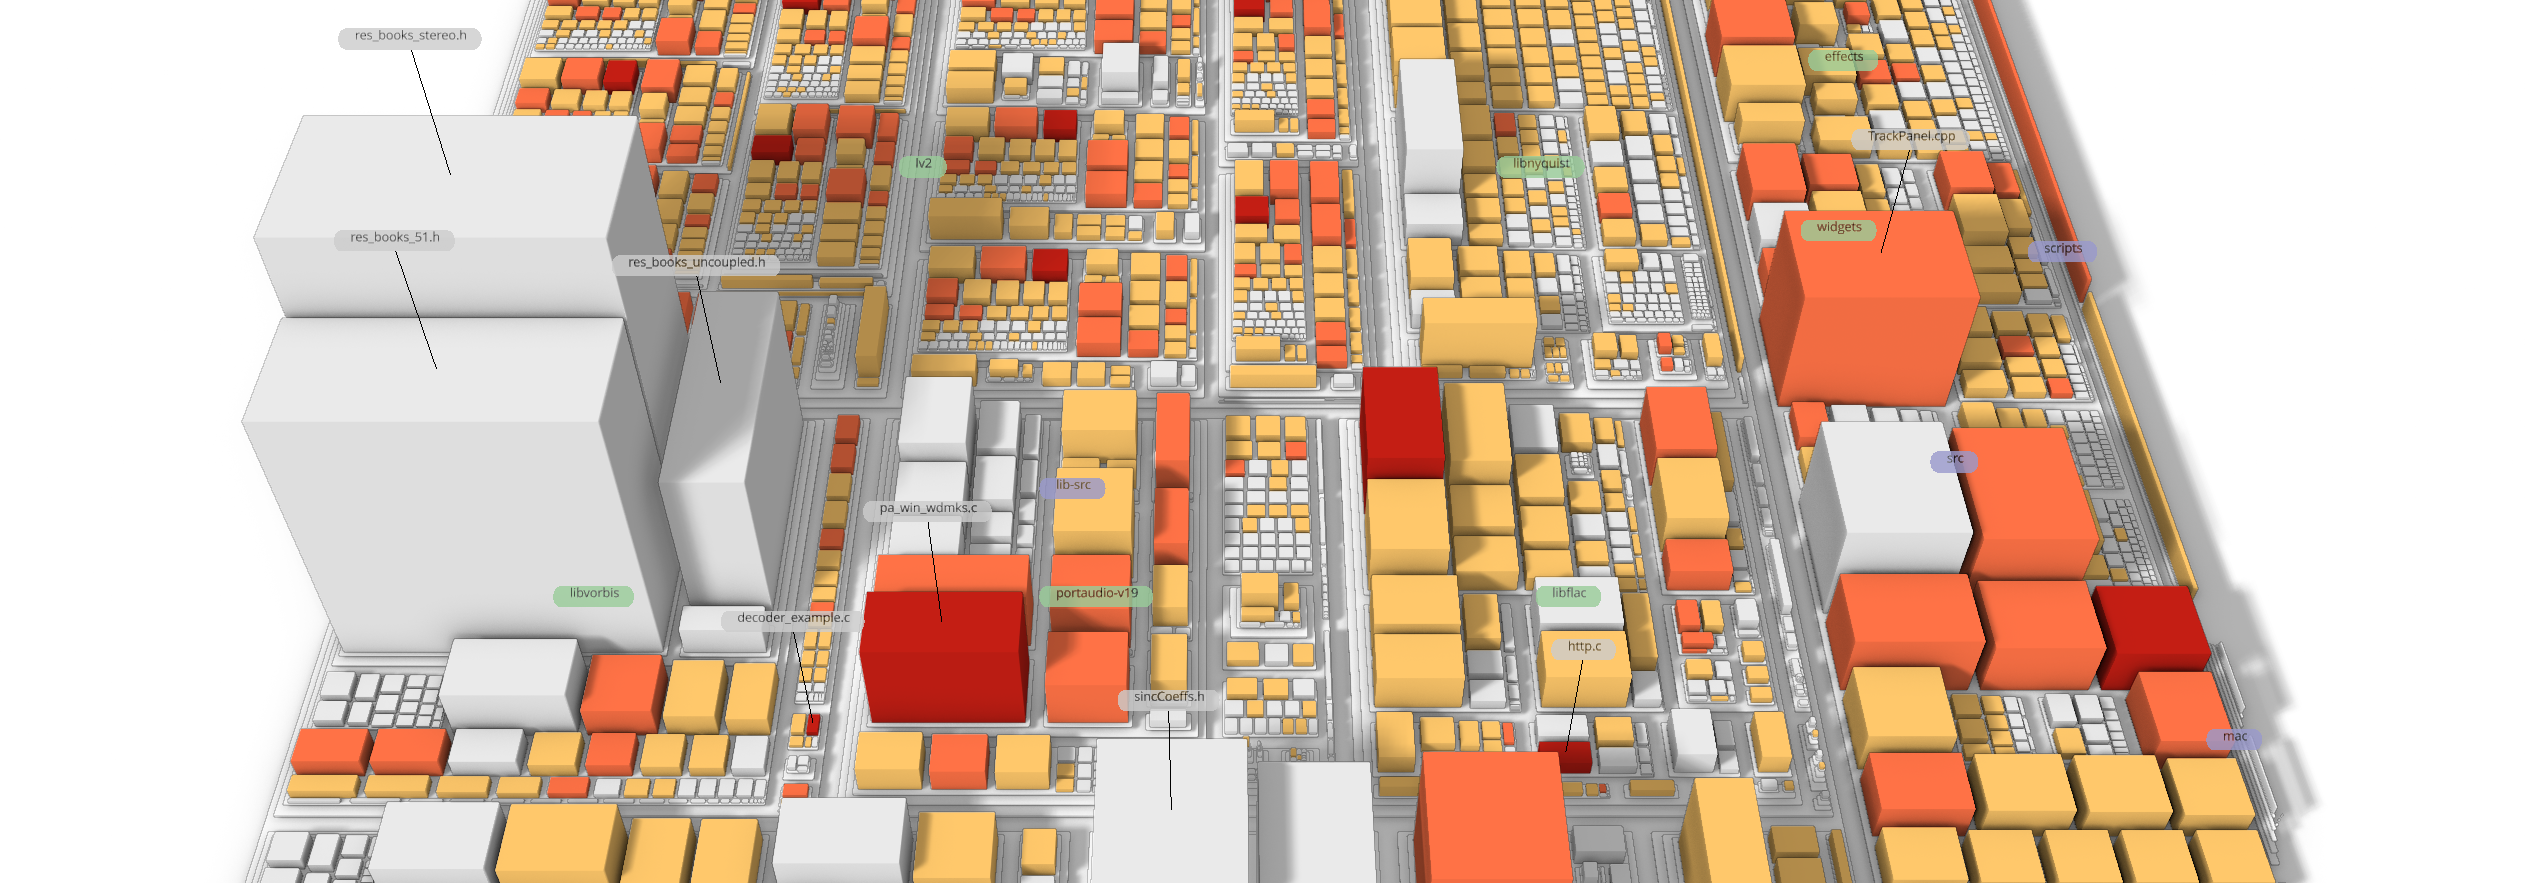
\includegraphics[height=0.278\textwidth]{images/audacity}
 	   \caption{Software map example: Audacity}
	\end{figure}
    
    \blueify{Rendering Service for Software Maps (Seerene)}
    
    \begin{itemize}
    	\item High-quality server-based 3D rendering of software maps
    	\item Scalable treemap rendering technique for massive tree data
    	\item Combined advanced rendering techniques (multi-sampling, shadows, ambient occlusion)
    \end{itemize}
    
\end{frame}


\begin{frame}{Computer Graphics Systems at HPI | \textbf{Built Systems 4/4}}
	
	\begin{figure}
		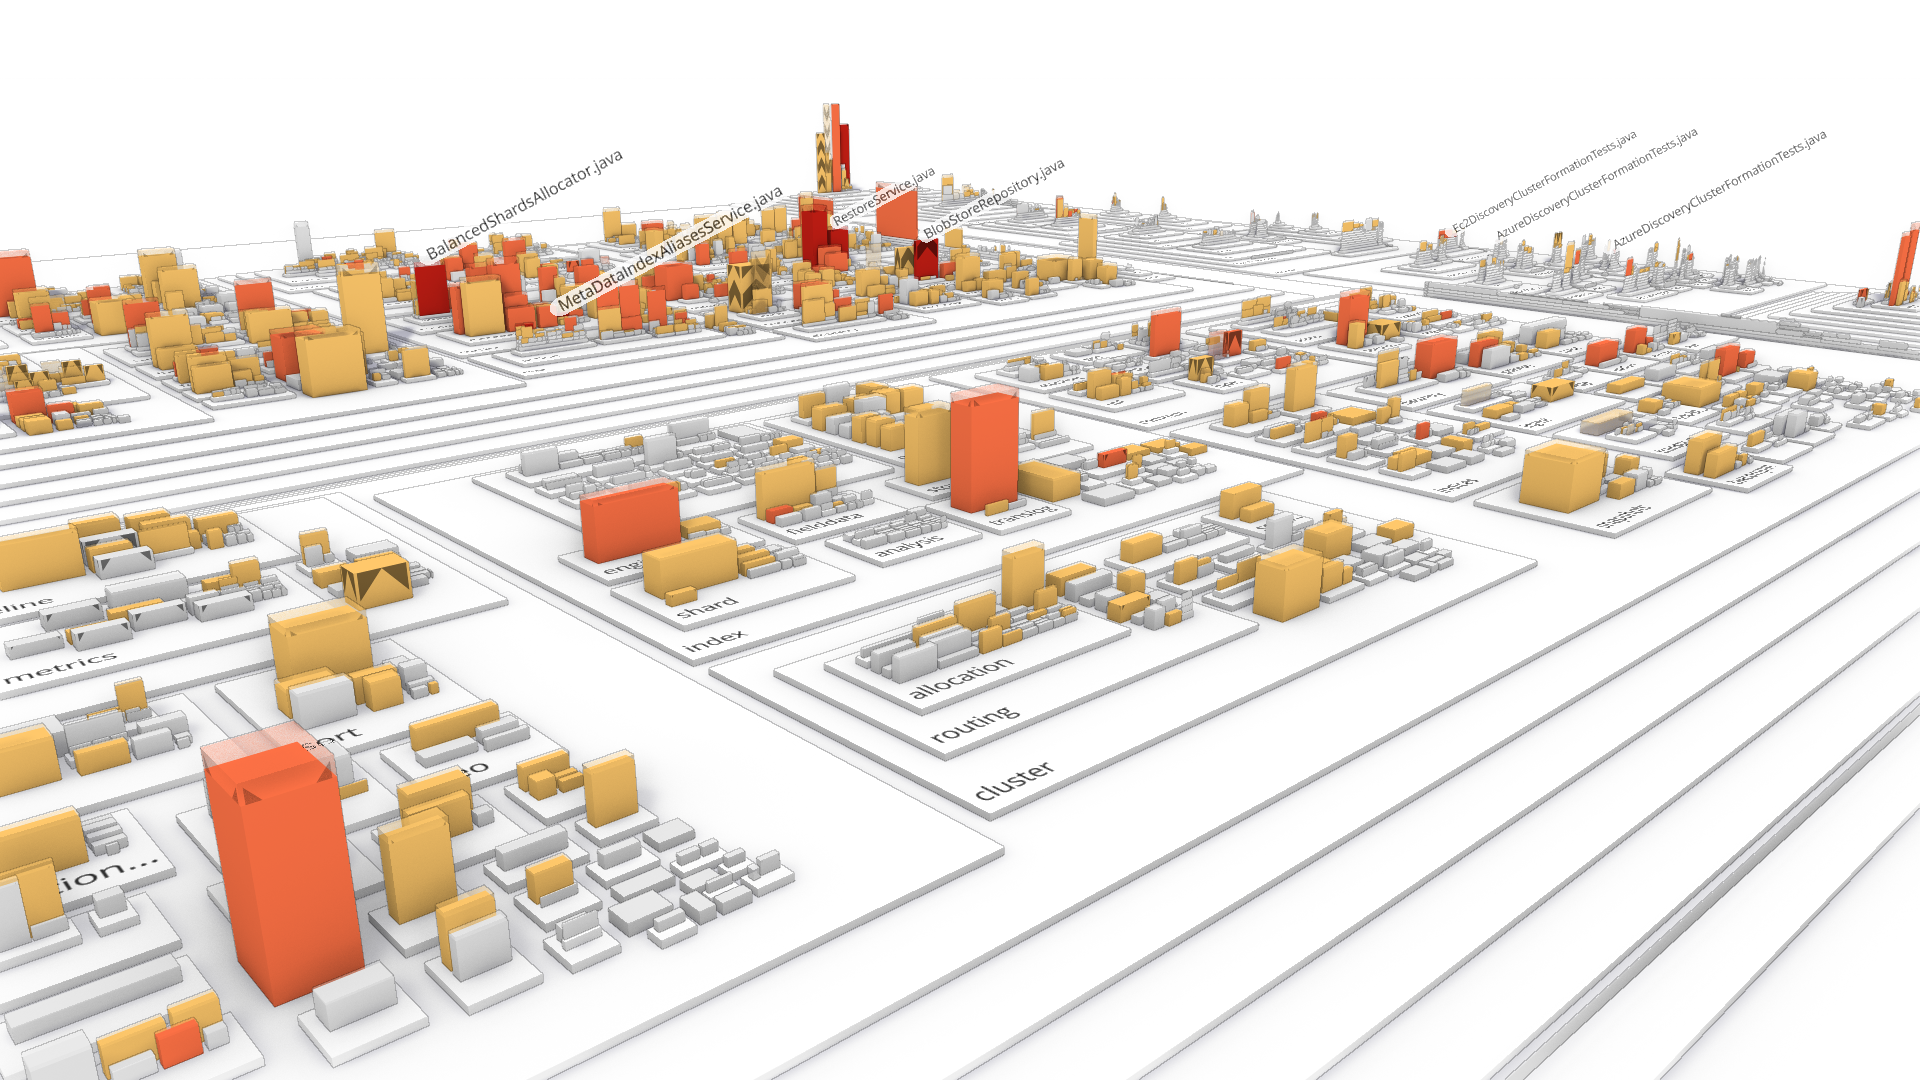
\includegraphics[width=0.35\textwidth]{images/arboretum}
		\hfill
		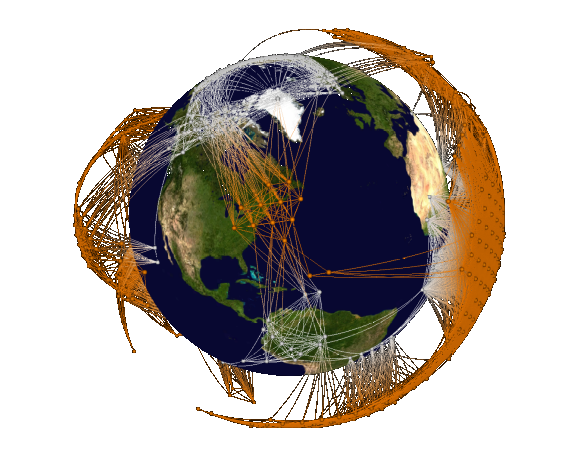
\includegraphics[width=0.25\textwidth]{images/gtx}
		\hfill
		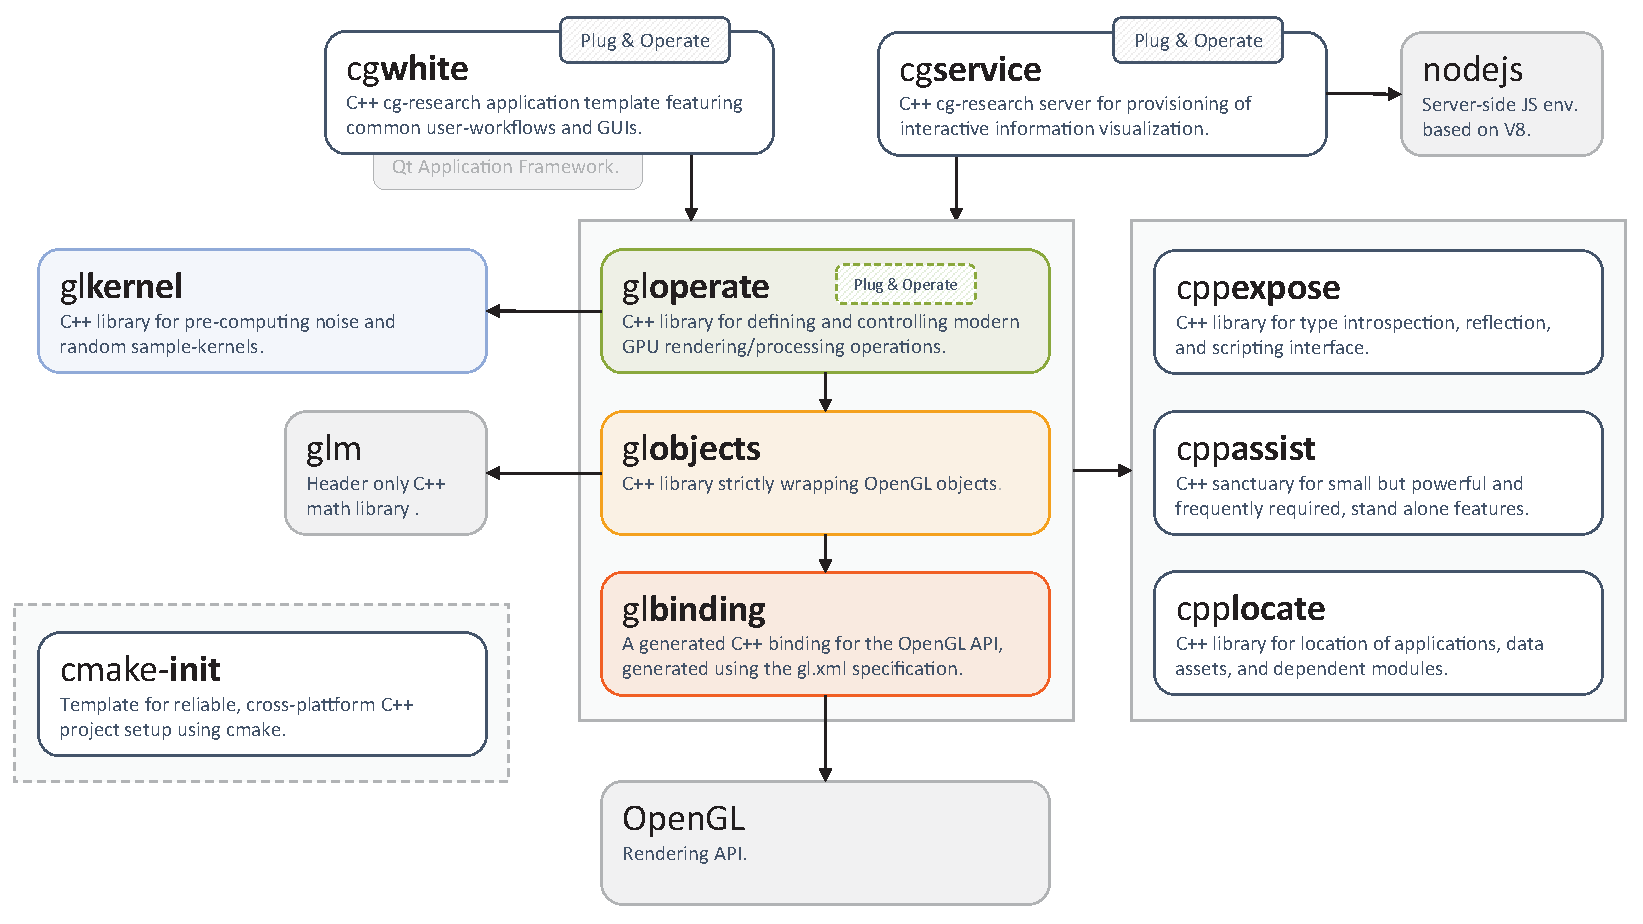
\includegraphics[width=0.34\textwidth]{images/middleware}
		\caption{Research prototype examples: Arboretum and GTX, both based on the gloperate rendering middleware}
	\end{figure}
	
	\blueify{CG Middleware (CG Internals) as base for research prototypes}
	
	\begin{itemize}
		\item Pipeline-based processing and rendering description
		\item Templates and recipes for visualization systems
		\item Modular software landscape and architecture (10 in-house libraries, 5 third-parties)
	\end{itemize}
	
\end{frame}